\paragraph{Exercice} $DL_3(0)$ de $e^{\sin x}$ ? \[e^{\sin x} = 1 + x + \frac{x^2}{2}+x^3\epsilon (x)\]

En effet, $\sin x = x - \frac{x^3}{6}+x^3 \epsilon (x)$. De plus, $\sin(0) = 0$ Donc on veut le DL de exp en 0 : \[
e^y = 1 + y + \frac{y^2}{2}+\frac{y^3}{6} + y^3 \epsilon (y)\]
Par composition, \[e^{\sin x} = 1 + (x-\frac{x^3}{6}) + \frac{1}{2}(x - \frac{x^3}{6})^2 + \frac{1}{6} (x - \frac{x^3}{6})^3 + x^3 \epsilon (x) \]

On obtient : \[\begin{array}{rcl}
e^{\sin x} &=& 1 + x - \frac{x^3}{6} + \overbrace{\frac{1}{2}(x^2)}^{\text{On a tronque}} + \overbrace{\frac{1}{6}x^3}^{\text{Ici aussi !}} + x^3\epsilon (x) \\
&=& 1 +x + \frac{x^2}{2} + 0x^3 + x^3 \epsilon (x)
\end{array}\]

\section{Applications des DL}
\subsection{Calcul de limites}
\[\begin{array}{rclr}
f(x) &=& \frac{e^x-1}{(1+x)^2 - 1} & lim \text{ en } 0 ? \\
&=& \frac{(1+x+x\epsilon(x)) -1}{x(x+2)} \\
&=& \frac{x(1+\epsilon(x))}{x(x+2)} &\text{ avec } \epsilon(x) \xrightarrow[x \to 0]{} 0 \\
&=& \frac{1+\epsilon(x)}{x+2} \xrightarrow[x \to 0]{} \frac{1}{2} & \text{ par opérations usuelles sur les limites } \end{array}\]

\paragraph{Exemple} $g(x) = \frac{1-\cos x}{x^2} = \frac{1-(1 - \frac{x^2}{2} + x^2 \epsilon(x))}{x^2} = \underbrace{\frac{1}{2} - \epsilon (x)}_{\xrightarrow[x \to 0]{} \frac{1}{2}}$

\[\begin{array}{rclr}
h(x) &=& \frac{\sqrt{2} - \sqrt{1+\cos x}}{\sin^2 x} & lim \text{ en } 0 \\
\sqrt{1+y} &=& 1 + \frac{1}{2} y - \frac{1}{8}y^2 + y^2 \epsilon (y) \\
\sqrt{1 + \cos x} = \sqrt{2+(\cos x - 1)} &=& \sqrt{2(1 + \frac{1}{2}(\cos x -))}\\
&=& \sqrt{2}(\sqrt{1+\frac{\cos x - 1}{2}}) \\
\frac{\cos x -1}{2} &=& \frac{1}{2}(-\frac{x^2}{2} + x^2 \epsilon (x)) = - \frac{x^2}{4} + x^2 \epsilon (x) \\
\text{D'ou } \sqrt{1+\frac{1}{2}(\cos x - 1)} &=& 1 + \frac{1}{2}\frac{-x^2}{4} + x^2 \epsilon (x) \\
&=& 1 - \frac{x^2}{8} + x^2 \epsilon (x) \\
\text{car } (\sin x)^2 &=& x^2 + x^2 \epsilon (x) \\
\text{Donc } h(x) &=& \frac{\sqrt{2} - \sqrt{2}(1-\frac{x^2}{8} + x^2 \epsilon (x))}{x^2 + x^2 \epsilon} \\
&=& \frac{x^2(\frac{\sqrt{2}}{8} + \epsilon (x))}{x^2(1+\epsilon x)} = \frac{\frac{\sqrt{2}}{8} + \epsilon (x)}{1+\epsilon (x)} \xrightarrow[x \to 0]{} \frac{\sqrt{2}}{8}
\end{array}\]

\paragraph{Remarque} $DL_N(x_0)$ de $gof$. ~\\
Il faut que :
\begin{itemize}
	\item $gof(x)$ existe pour $x \in ]x_0 - \delta; x + \delta[$. ~\\
	\item f admette un $DL_n(x_0)$
	\item g admette un $DL_n$ en $f(x_0)$
\end{itemize}

\subsection{sign local d'une fonction}
\paragraph{Proposition} $f : I \rightarrow \mathbb{R}$, I intervalle de $\mathbb{R}$, si $f(x) = c(x-x_0)^n + (x-x_0)^2 \epsilon (x)$ avec $C \neq 0, \epsilon (x) \xrightarrow[x \to x_0]{} 0$ ~\\
\begin{tabular}{cc|c}
& n pair & n impair \\
$c > 0$ & {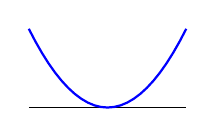
\begin{tikzpicture}
\draw[] (-1, 0) -- (1, 0);
\draw[blue, thick, domain=-1:1] plot(\x, {\x*\x});
\end{tikzpicture}} & {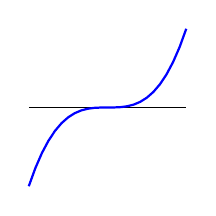
\begin{tikzpicture}
\draw[] (-1, 0) -- (1, 0);
\draw[blue, thick, domain=-1:1] plot(\x, {\x*\x*\x});
\end{tikzpicture}} \\
\hline
$c < 0$ &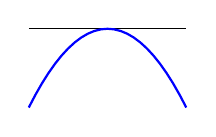
\begin{tikzpicture}
\draw[] (-1, 0) -- (1, 0);
\draw[blue, thick, domain=-1:1] plot(\x, {-\x*\x});\end{tikzpicture} & 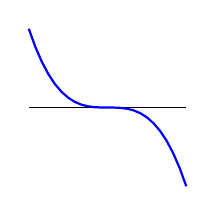
\begin{tikzpicture}
\draw[] (-1, 0) -- (1, 0);
\draw[blue, thick, domain=-1:1] plot(\x, {-\x*\x*\x});
\end{tikzpicture}
\end{tabular}

\begin{wrapfigure}[4]{r}{0pt}
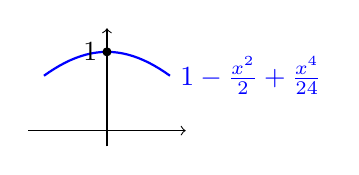
\begin{tikzpicture}

\draw[->] (-1, 0) -- (1, 0);
\draw[->] (0, -0.2) -- (0, 1.3);
\draw[blue, thick, domain=-0.8:0.8] plot(\x, {cos(\x r)}) node[right] {$1-\frac{x^2}{2} + \frac{x^4}{24}$};
\draw[fill=black] (0, 1) circle (0.05) node [left] {$1$};

\end{tikzpicture}
\end{wrapfigure}

\paragraph{Exemple} $\cos x = 1 - \frac{x^2}{2} + \frac{x^4}{24} + x^4 \epsilon (x)$ avec $\epsilon (x) \xrightarrow[x \to 0]{} 0$~\\ ~\\
\[\begin{array}{rcl}
\text{En particulier :  } (\cos x -1) &=& - \frac{x^2}{2} + x^2 \epsilon (x) \\
&=& \underbrace{-\frac{1}{2} x^2 + x^2 \epsilon (x)}_{x=2 : \text{ pair }} \\
c&=& -\frac{1}{2} < 0 \\
\\
\text{De plus, } \cos x - (1-\frac{x^2}{2}) &=& \underbrace{\frac{1}{24}}_{c > 0}x^{\overbrace{4}^{\text{n pair}}} + x^4\epsilon (x) \\
\end{array}\]

\begin{center}

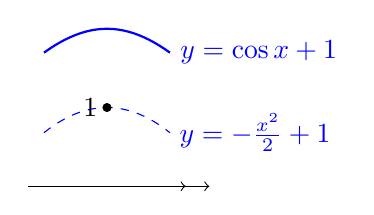
\begin{tikzpicture}
\draw[->] (-1, 0) -- (1, 0);
\draw[->] (0, 0) -- (1.3, 0);
\draw[blue, thick, domain=-0.8:0.8] plot(\x, {cos(\x r) +1}) node [right]{$y = \cos x + 1$};
\draw[blue, dashed, domain=-0.8:0.8] plot(\x, {-\x*\x / 2 +1}) node [right]{$y = -\frac{x^2}{2} + 1$};
\draw[fill=black] (0, 1) circle (0.05) node [left] {$1$};

\end{tikzpicture}

\end{center}


\begin{wrapfigure}[5]{r}{0pt}
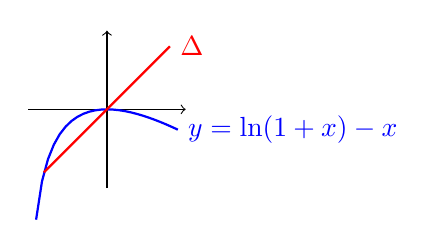
\begin{tikzpicture}

\draw[->] (-1, 0) -- (1, 0);
\draw[->] (0, -1) -- (0, 1);
\draw[blue, thick, domain=-0.9:0.9] plot(\x, {ln(1+\x)-\x}) node [right]{$y = \ln(1+x) - x$};
\draw[red, thick] (-0.8, -0.8) -- (0.8, 0.8) node[right] {$\Delta$};

\end{tikzpicture}
\end{wrapfigure}
\paragraph{Exemple} $x \mapsto \ln(1+x)$ ~\\
Sa tangeante en 0 est la droite $\Delta : y=x$. De plus, $\ln(1+x) = x + -\frac{x^2}{2} + x^2 \epsilon(x)$

Donc $\ln (1+x) -x = -\frac{1}{2}x^2 + x^2 \epsilon(x)$

\subsection{Position par rapport à une asymptote}

\begin{wrapfigure}[5]{r}{0pt}

	\begin{tikzpicture}
		\draw[->] (-2, 0) -- (2, 0);
		\draw[->] (0, -2) -- (0, 2);
		\draw[blue, thick, domain=-2:2] plot(\x, {\x /2 - 1 / 4}) node [right]{$\Delta$};
		\draw[red, domain=-2:2] plot(\x, {x/2 * (1-1/\x - 1 / (4*\x*\x))}) node [right] {$y=f(x)$};
	\end{tikzpicture}

\end{wrapfigure}

\paragraph{Exemple} $f(x) = \frac{x^3}{1+x+2x^2}$

\[\begin{array}{rclr}
f(x) &=& \frac{x^3}{2x^2}(\frac{1}{\frac{1}{2x^2} + \frac{1}{2x}+1}) \\
	&=& \frac{x}{2}(\frac{1}{1+(\frac{1}{2x}+\underbrace{\frac{1}{2x^2}}_{u})})} \\
u(y) &=& \frac{1}{2}y + \frac{1}{2}y^2 & \text{ avec } y = \frac{1}{2} \\
\frac{1}{1+u} &=& 1-u+u^2+u^3 \epsilon (u) \\
&=& 1 - (\frac{1}{2x} + \frac{1}{2x^2}) + (\frac{1}{2x} + \frac{1}{2x^2})^2 +  \frac{1}{x^2}\epsilon(\frac{1}{x}) \\
&=& 1 - \frac{1}{2x} - \frac{1}{2x^2} + \frac{1}{4x^2} + \frac{1}{x^2}\epsilon(\frac{1}{x}) \\
&=& 1 - \frac{1}{2x} - \frac{1}{4x^2} + \frac{1}{x^2} \epsilon (\frac{1}{x})
\\
f(x) &=& \frac{x}{2}(1-\frac{1}{2x}-\frac{1}{4x^2}+\frac{1}{x^2}\epsilon (x)) \\
&=& \frac{x}{2} - \frac{1}{4} - \frac{1}{8x} + \frac{1}{x}\epsilon (x) \\
&=& \frac{x}{2} - \frac{1}{4} - \frac{1}{8x} + \frac{1}{x}\epsilon (x) \\
f(x) - (\frac{x}{2}-\frac{1}{4}) &=& \underbrace{-\frac{1}{8x} +  \frac{1}{x}\epsilon (x) }_{\text{asymptote}} \xrightarrow[x \to \pm \infty]{} 0 \\
\Delta &=& y & \frac{1}{2}x - \frac{1}{4};
\end{array}\]

